%%% Preamble
  \documentclass[a4paper, 11pt, twoside]{article}
  \usepackage[T1]{fontenc}
  \usepackage{fourier}
  \usepackage[english]{babel}
  \usepackage[protrusion=true,expansion=true]{microtype}
  \usepackage{amsmath,amsfonts,amsthm}
  \usepackage[pdftex]{graphicx}
  \usepackage{url}
  \usepackage{setspace}
  \usepackage{vmargin}
  \setmarginsrb {0.79in}  % left margin
                {1.00in}   % top margin
                {0.79in}   % right margin
                {0.79in}  % bottom margin
                {  20pt}   % head height
                {0.25in}   % head sep
                {   9pt}    % foot height
                { 0.3in}    % foot sep

  \usepackage{sectsty}
  \allsectionsfont{\centering \normalfont\scshape}

  % Bibliography
  \usepackage{natbib}
  \bibliographystyle{aer}
  \setlength{\parindent}{0.25in}


  %% Added by me
  \usepackage{pdfpages}
  \usepackage{booktabs}
  \usepackage{wrapfig}
  \usepackage{float}
  \usepackage{pdfsync}
  \usepackage{fancyhdr}
  \usepackage{multicol}
  \newcommand\ve{\varepsilon} % From Rick
  \theoremstyle{definition} % From Rick
  \newtheorem{definition}{Definition} % Number definitions on their own
  \usepackage{hyperref}  % From Rick
  \hypersetup{colorlinks,linkcolor=cyan,urlcolor=blue,citecolor=black}
  \usepackage{colortbl}
  \usepackage{caption}

  %%% Equation and float numbering
  \numberwithin{equation}{section}

  %% EVEYTHING BELOW NEEDS TO BE CHANGED!
  %% Setup default header
  \fancypagestyle{mainDoc}{
      \fancyhead[L]{\small Lyon: TSA Equity Premium Puzzle}
      \fancyhead[R]{\thepage}
      \fancyfoot{} % no footer
      \renewcommand{\headrulewidth}{.5pt}
      \renewcommand{\footrulewidth}{0pt}
      \setlength{\headheight}{13.6pt}
  }

  %%% Maketitle metadata
  \newcommand{\horrule}[1]{\rule{\linewidth}{#1}}     % Horizontal rule

  % Set title here
  \newcommand \thetitle{Time Series Analysis of the Equity Premium Puzzle}

  \title{
    \vspace{-.6in}
    \usefont{OT1}{bch}{b}{n}
    \normalfont \normalsize \textsc{ } \\ [25pt]
    \horrule{0.5pt}
    \huge \thetitle \\
    \horrule{2pt}
  }

  \author{
    Spencer Lyon
    % \thanks{}
  }

  \date{
  \normalfont \normalsize
  \today \\[-4pt] \normalsize
  }

  \newcommand{\TODO}[1]{ {\color{magenta} TODO: #1} }

%% Title Page
\begin{document}
\begin{titlepage}
  \maketitle
  \thispagestyle{empty}
  \begin{center}

  \includegraphics{logo} \\ [0.8cm] % University/department logo - uncomment to place it

  Macroeconomics and Computational Laboratory (MCL) \\[0.5cm] % Research group name
  BYU Economics\\[1.5cm]  % and department name

  % \large{\textit{Abstract}}
  \begin{abstract}
      \normalsize
      \setstretch{1.}
        This paper analyzes the age-old question of the equity premium puzzle (EPP) from the perspective of time series models. The EPP addresses the question for why demand for risky assets is so low compared to risk-free assetes when the expected returns on risky assets are so much higher. I estimate that the equity premium between 1990-2012 is between 3.4-5.2\%. I use ARIMA and GARCH models to forecast data and find that the forecasted equity premium is between 1.2-3.8\%.
  \end{abstract}
  \end{center}
  \tableofcontents
\end{titlepage}

%% Main document
\newpage
\pagenumbering{arabic}  % Use arabic numbers now
\setcounter{page}{1}  % Reset page numbering

\begin{center}
\huge{\thetitle}  % Make sure the newcommand \thetitle is defined above
\rule{\linewidth}{.1pt}
\end{center}

\setstretch{1.75}

\section{Introduction} \label{sec:intro}
  \thispagestyle{empty}
  \pagestyle{mainDoc}

  One longstanding phenomenon economists see in financial data is known as the equity premium puzzle \citep{Prescott:1985}. The heart of the equity premium puzzle can be summarized one of two equivalent questions: why is demand for risk free government bonds so high when returns on those assets are so low? The second question could be stated as follows:  why is demand for stocks, and hence stock prices, so low despite the relatively high expected returns

  Over the years economists have posed many possible explanations for why the equity puzzle premium (EPP) exists, or even if it exists. Modern economics is based largely on rational expectations and risk aversion. An appeal to these theories to explain the EPP seems natural and intuitive; however, this type of explanation falls very short. To put this disparity in perspective \cite{Mankiw:1991} pointed out that in order for risk aversion to explain the EPP, investors would have to be indifferent between taking a sure \$51,209 or having 50\% at winning either \$50,000 and \$100,000. Other common explanations have generally been rooted in tax policy, market failures, liquidity constraints, and the implied volatility of the underlying equities.

  The focus of this paper will be analyzing the ability of ARIMA and (G)ARCH models for identifying and explaining the equity premium puzzle. ARMIA methods have been around for some time and have held a significant foothold in the finance literature.  An ARIMA model allows the economist to model the effect of historical moving averages on current values. This flexibility is particular appealing to someone trying to model financial time series because things like seasonality, momentum, and market lags and/or inefficiencies lead to these moving averages storing a lot of relevant data.

  ARCH and GARCH models are, in a sense, very similar to ARIMA models. Instead of trying to model the effect of changing moving averages, (G)ARCH models attempt to capture changes in the variance of underlying parameters. It is immediately apparent the trained financial eye that focusing on the changes in expected variance might actually be more instructive than moving averages when applied to forecasting models.

  The remainder of this paper will be structured as follows: Section ~\ref{sec:estimation} will discuss ARIMA and (G)ARCH models as well as the data I am using, Section~\ref{sec:estimatingreturns} will show the results of my analysis, and Section~\ref{sec:conclusion} will have a few concluding thoughts and ideas for further research.

\section{Estimation} \label{sec:estimation}

  \subsection{The Data} \label{sub:the_data}

    The data for this paper is quite simple. To mimic a risk free asset I have gathered daily data for the price of both 3-month and 10-year US treasury bills. I obtained this data from the St. Louis Federal reserve under the data set names DGS3MO and DGS10 for the 3-month and 10-year maturities, respectively. The units on these data sets are percent returns, the data is not seasonally adjusted, and the data was sampled at a daily frequency.

    To model risky assets I chose to use the daily returns on the S\&P 500 stock market index.  The units on this data set is US dollars (\$) and I retrieved the data from Yahoo! Finance. The S\&P 500 was a natural choice because it is a very common metric used in finance to measure the overall movement of the stock market. Because some explaination of the EPP refer to the volatility of stocks I also chose to use the VIX, also from Yahoo! Finance. \footnote{The VIX is constructed using the implied volatilities on call and put options for the stocks making up the S\&P 500. It is the generally accepted measure of overall stock market volatility.}

    For the most part, these four time series had observations on the same days: all of them are reported for week-days only. However, the big difference is that the data from Yahoo! Finance is only reported on trading days, while the data from FRED is reported every Monday through Friday, including most holidays. To overcome this I simply dropped observations for days where FRED reported data, but the stock markets were closed. In Table ~\ref{tab:describe} I have included a summary of this data and a simple plot of the data in Figure ~\ref{fig:alldata}.

    \setstretch{1.2}
    \begin{figure}[ht]
        \centering
        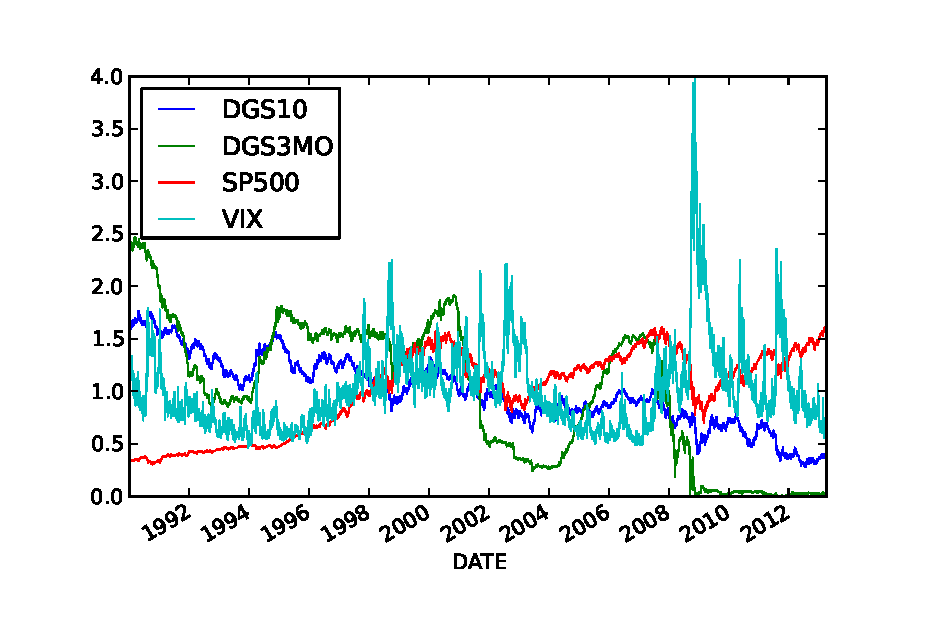
\includegraphics[width=6in]{./Figures/all_data.eps}
        \captionsetup{width=5.5in}
        \caption{\small Plot of the data used in this paper. Note that because the units are different and the value of the S\&P 500 is much larger than the percents on the T-bill data sets, I have divided each data set by its mean before plotting.}
        \label{fig:alldata}
    \end{figure}

    \begin{table}[ht!]
      \begin{center}
        \begin{tabular}{r|ccccc}
        \hline
           \rowcolor{gray!45}  & DGS10  (\%)& DGS3MO  (\%)& SP500 (\$)& VIX (\$)\\
          \hline
          \hline
          \rowcolor{gray!7} obs & $5814$ & $5814$ & $5814$ & $5814$\\
          \rowcolor{gray!23}mean & $5.13971$ & $3.34731$ & $971.369$ & $20.3545$\\
          \rowcolor{gray!7} std & $1.72623$ & $2.25087$ & $375.187$ & $8.09241$\\
          \rowcolor{gray!23}min & $1.43$ & $0$ & $295.46$ & $9.31$\\
          \rowcolor{gray!7} 25\% & $3.98$ & $1.17$ & $585.983$ & $14.62$\\
          \rowcolor{gray!23}50\% & $5.06$ & $3.69$ & $1091.49$ & $18.755$\\
          \rowcolor{gray!7} 75\% & $6.37$ & $5.14$ & $1283.34$ & $23.87$\\
          \rowcolor{gray!23}max & $9.09$ & $8.26$ & $1587.73$ & $80.86$\\
        \bottomrule
        \end{tabular}
        \captionsetup{width=5.5in}
        \caption{\small Summary of the data . All the data was sampled from 1/1/2000 to 3/28/2013. Note the rows with percent labels correspond to percentiles}
        \label{tab:describe}
      \end{center}
    \end{table}
    \setstretch{1.75}

  \newpage
  \subsection{ARIMA Models} \label{sub:arima}

    Time series modeling is all about identifying time-varying trends in data and extrapolating those trends into the future with as little error as possible. One very general family of time series models is known as the ARIMA model, or autoregressive integrated moving average model. There are at least three roles an ARIMA model (or any forecasting model) can play:

    \begin{enumerate}
      \item By themselves to predict future values of a dependent variable
      \item To predict the future value of an independent variable in an economic model
      \item To estimate future values of systematic residuals in an economic model
    \end{enumerate}

    In this paper I will be using ARIMA models within the first category listed above. In order to understand how I will be using them I will first explain what the model is in a general form. An ARIMA model is defined in terms of three parameters $p, q, \text{ and }, d$ and is defined as follows:

    \setstretch{1.2}
    \begin{align}
     Y_t^* - \phi_1Y_{t-1}^*  - \dots - \phi_pY_{t-p}^* &= \ve_t - \theta_1\ve_{t-1} - \dots - \theta_q \ve_{t-q} \label{eq:arimalong}\\
     \left( 1 - \sum_{i=1}^p \phi_i L^i\right) Y_t^* &= \left( 1 + \sum_{i=1} ^q \theta_i L^i \right) \ve_t \label{eq:arima}
    \end{align}

    \setstretch{1.75}
    Where $L$ is the lag operator and $Y_t^* \equiv (1 - L)^d Y_t$. A slightly different form of the ARIMA equation allows for an additional "drift" term $ \delta$ that can be thought of as an intercept term for the errors. This modified form appears below.

    \setstretch{1.2}
    \begin{align}
      \left( 1 - \sum_{i=1}^p \phi_i L^i\right) Y_t^* &= \delta + \left( 1 + \sum_{i=1} ^q \theta_i L^i \right) \ve_t \label{eq:arimadrift}
    \end{align}

    \setstretch{1.75}
    \subsubsection{Identification} \label{ssub:identification}

      The first major roadblock when trying to build an ARIMA model is identifying the parameters $p, q, \text{ and } d$. I will start by trying to identify $p$ and $q$. To do this I need to look at the autocorrelation and partial autocorrelation coefficients (see McDonald notes section 8). In Figure~\ref{fig:correlations} I have included a plot of the autocorrelation and partial autocorrelation coefficients for each data set.

      \begin{figure}[!h]
        \centering
        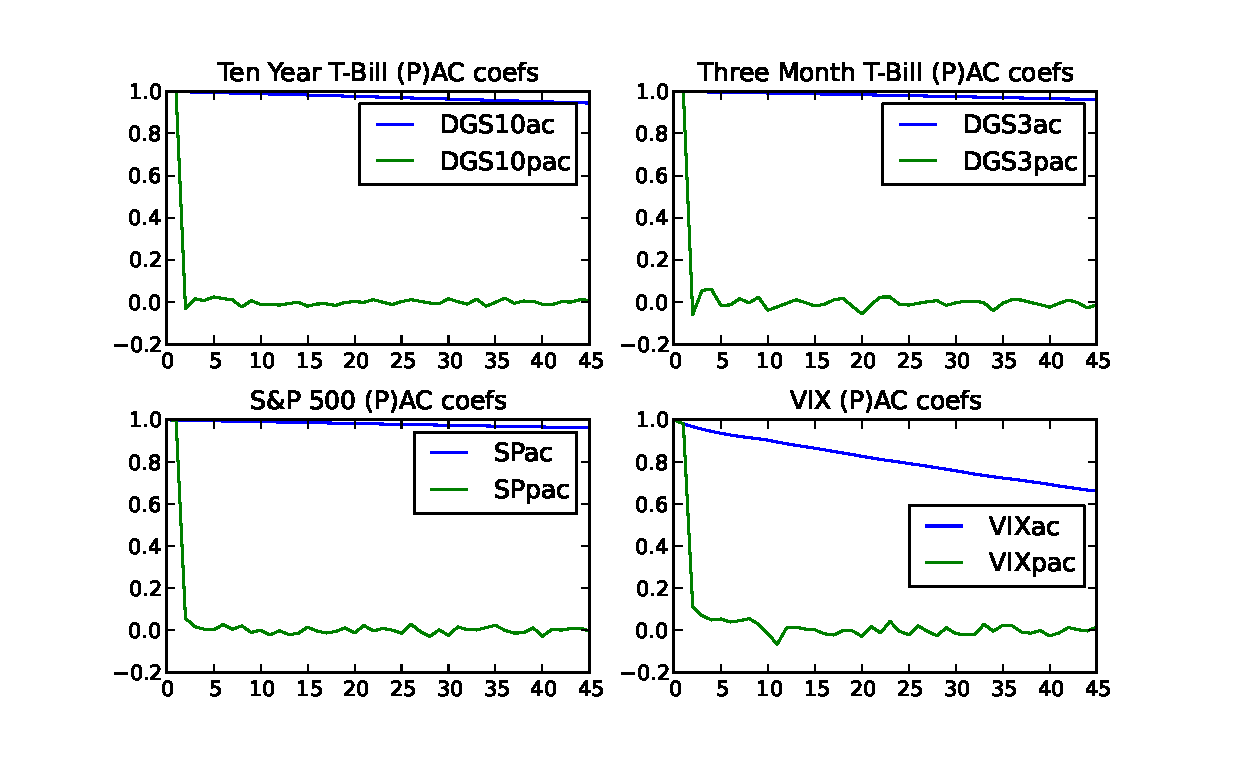
\includegraphics[width=6in]{./Figures/all_corrs.eps}
        \captionsetup{width=5.5in}
        \caption{\small Autocorrelation and partial autocorrelation coefficients for each data set. Used to find the parameters $q$ and $p$ in an ARIMA model. The initial spike in the partial autocorrelation coefficients and the gradual descent of the autocorrelation coefficients suggets $p=1$, and $q=0$.}
        \label{fig:correlations}
      \end{figure}

      As can be clearly seen, for each of my time series we have an initial spike in the partial autocorrelation coefficient for 1 lag and then nothing. Also, in each picture we see that the autocorrelation coefficients slowly decline for all 4 time series. Together, these two pieces of information suggest that we should approximate an AR(1) model by setting $p = 1 $and $q = 0$. Another important feature in each of this plots is that while the decrease in the autocorrelation coefficients is steady, it is also very slow. This is indicative of a need to difference the data to make it more stationary before applying the model.

      The last identification step is to determine a suitable value for d, or determine how many times the data needs to be differenced before it is stationary. This is a bit more subjective, but can still be formalized. I used two different techniques to do this. The first is taking successive differences of the data, looking at plots and the first two moments and stopping when the data looks stationary.  In Table~\ref{tab:differences} I have included a table that reports the mean and variance of the first 4 differences for all 4 data sets.

      \begin{table}[h!]
        \begin{centering}
        \setstretch{1.25}
        \begin{tabular}{|l|c|cc||l|c|cc|}
          \hline
           \rowcolor{gray!45} DataSet & Lags &   Mean &     Variance & DataSet & Lags &   Mean &     Variance \\
          \hline
          \hline
           \rowcolor{gray!7} DGS10  & 1    & -0.0014 &  0.0039 & SP500  & 1    &   0.0344 &  224.2908 \\
           \rowcolor{gray!23} {} &     2    & -0.0028 &  0.0079 & {} &     2    &   0.0839 &  406.3557 \\
           \rowcolor{gray!7} {} &     3    &  -0.0042 &   0.0115 & {} &      3    &    0.1329 &   574.528 \\
           \rowcolor{gray!23} {} &     4    & -0.0056 &   0.0151 & {} &     4    &    0.1779 &  748.1064 \\
           \rowcolor{gray!7} DGS3MO &  1    & -0.0016 &  0.0033 & VIX    & 1    & -0.0034 &   3.1320 \\
           \rowcolor{gray!23} {} &     2    & -0.0032 &  0.0077 & {} &     2    & -0.0076 &  5.3557 \\
           \rowcolor{gray!7} {} &     3    &  -0.0048 &   0.0114 & {} &     3    &  -0.0118 &  7.2619 \\
           \rowcolor{gray!23} {} &     4    & -0.0064 &   0.0140 & {} &     4    &  -0.0154 &  9.0184 \\
          \hline
        \end{tabular}
        \captionsetup{width=5.5in}
        \caption{Mean and Variance of data sets for first 4 lags for each time series. The goal is stationarity, so the correct number of lags will have a small mean and variance.}
        \label{tab:differences}
        \end{centering}
      \end{table}
      \setstretch{1.75}

      The second method for determining the correct number of lags is to use an augmented Dickey Fuller test.  the augmented Dickey Fuller (ADF) test is used to check for unit roots in a time series. In other words, the ADF test is applied to a time series to see if in a regression of the time series on its first lag produces a coefficient equal to 1 (exact correlation with previous period data - could be a random walk). The null hypothesis in the ADF test is that there is a unit root. I performed the ADF for all four data sets for the data by itself as well as the first lag. The results appear in Table ~\ref{tab:dickeyfuller}.

      \begin{table}
        \begin{centering}
        \setstretch{1.25}
          \begin{tabular}{|l|l|cc|}
          \hline
            \rowcolor{gray!45} DataSet & Lags &  Statistic & p-value\\
            \hline
            \hline
            \rowcolor{gray!7} SP500 & 0 & -1.8564 & 0.6391\\
           \rowcolor{gray!23} {} & 1  & -18.0968 & 0.0001\\
            \rowcolor{gray!7} VIX & 0 & -4.9092 & 0.0001\\
           \rowcolor{gray!23} {} & 1  & -19.162 & 0.0001\\
            \rowcolor{gray!7} DGS10 & 0 & -3.9125 & 0.0133\\
            \rowcolor{gray!23} {} & 1 & -16.5723 & 0.0001\\
            \rowcolor{gray!7} DGS3MO & 0 & -1.5736 & 0.7589\\
            \rowcolor{gray!23} {} & 1 & -17.1829 & 0.0001\\
          \bottomrule
          \end{tabular}
          \setstretch{1.75}
          \captionsetup{width=5.5in}
          \caption{Results from the augmented Dickey-Fuller test. The test was run for each data set with no lags and again with a single lag. The test statistic corresponding to the 5\% confidence level is $ -3.5$. Any statistic lower than that suggests that the data might already be stationary (hence the small p-value).}
          \label{tab:dickeyfuller}
        \end{centering}
      \end{table}

      The null hypothesis associated with the ADF test is that there exists a unit root, or that the data is not stationary. We can see that we fail to reject that hypothesis at the $\alpha = 0.05$ level for the SP500 and DGS10 data sets without differencing the data. We can, however safely reject that hypothesis for all data sets after differencing one time. For uniformity, we will use one difference for each data set.  In summary, we will be using an ARIMA(1, 1, 0) model for all 4 data sets.

    \subsubsection{Evaluation} \label{ssub:evaluation}

      After the identification comes the evaluation of the model coefficients. I used the statistical programming language R and its forecast package\footnote{R is an open-source, but very complete and robust statistical package. It can be found at \url{http://cran.r-project.org/}.}. The results of the regressions are in Table ~\ref{tab:arimasum}.

      \begin{table}[h!]
        \begin{centering}
        \setstretch{1.25}
          \begin{tabular}{|l|l|cc|}
          \hline
            \rowcolor{gray!45} DataSet &  Statistic & Value & Standard Error\\
            \hline
            \hline
            \rowcolor{gray!7} SP500  & ar1   & -0.076882 &   0.0131 \\
            \rowcolor{gray!23} {} &   drift &  0.295485 &   0.1502 \\
            \rowcolor{gray!7} VIX   &  ar1   & -0.120370 &   0.0130 \\
            \rowcolor{gray!23} {} &   drift &  0.005510 &   0.0181 \\
            \rowcolor{gray!7} DGS10  & ar1   &  0.032490 &   0.0131 \\
            \rowcolor{gray!23} {} &  drift &  0.001087 &   0.0008 \\
            \rowcolor{gray!7} DGS3MO & ar1   &  0.114742 &   0.0131 \\
            \rowcolor{gray!23} {} & drift &  0.000613 &   0.0008 \\
          \bottomrule
          \end{tabular}
          \setstretch{1.75}
          \captionsetup{width=5.5in}
          \caption{Results from each of the ARIMA estimations. The coefficients on each term as well as the standard errors appear in the table.}
          \label{tab:arimasum}
        \end{centering}
      \end{table}

      Once I had the ARIMA model identified and estimated I simply needed to come up with forecasts for each data set. Again, I allowed the forecast package in R to do this for me. I forecasted the data out 1,500 additional observations. I felt that this was reasonable because I had almost 6,000 observations for each series.

  \subsection{(G)ARCH Models} \label{sub:garch}

    ARCH and GARCH models take a slightly different approach to time series modeling. Instead of trying to capture time varying trends in the expected value of a time series (like in ARIMA models), (G)ARCH models attempt to identify and measure time dependent trends in the volatility (or variance) of the data. (G)ARCH stands for (generalized) autoregressive conditional heteroskedasticity and allows for the current error term in the model to be a function of the error terms in previous periods.

    ARCH models were first introduced by \cite{Engle:1982} and GARCH models were introduced a few years later by \cite{Bollerslev:1986}. Both have been have been very popular in modeling financial and economic data\footnote{On April 13, 2013 a google search for "ARCH finance" returned over 20 million results in 0.20 seconds}. The variance for an ARCH($q$)model can be obtained from the following equation:

    \setstretch{1.2}
    \begin{align}
      \sigma^2_t = \alpha_0 +  \sum_{i=i}^q \alpha_i \ve_{t-i}^2 \label{eq:arch}
    \end{align}

    \setstretch{1.75}
    In equation \eqref{eq:arch} $\ve_t$ represents the residuals for the data in period $t$, $\sigma_t$ is the variance for the data in period $t$, and the $\alpha$'s  are coefficients for the residuals. The variance for a GARCH($q, p$) model is the same as  the ARCH($q$) model, except that it allows the variance in period $t$ to be a function of the variance in previous periods. This equation appears below appears below:

    \setstretch{1.2}
    \begin{align}
      \sigma^2_t = \alpha_0 +  \sum_{i=i}^q \alpha_i \ve_{t-i}^2 + \sum_{j=1}^p \delta_j\sigma_{t - j}^2 \label{eq:garch}
    \end{align}

    \setstretch{1.75}
    Before jumping into the estimation I felt it was necessary to test for arch effects. Table ~\ref{tab:archlm} shows the results of the LM test for arch effects for each of the data sets. The ARCH LM test operates under the null hypothesis that there are no ARCH effects. We can clearly see  (look at the p-values) that this hypothesis should be rejected for all data sets, or that we should assume there are arch effects in our data.

    \begin{table}[ht!]
      \begin{center}
        \begin{tabular}{r|ccccc}
        \hline
           \rowcolor{gray!45}  & DGS10  & DGS3MO  & SP500 & VIX \\
          \hline
          \hline
          \rowcolor{gray!7} $\chi^2$ & $5680.246$ & $5789.763$ & $5752.554$ & $5120.435 $\\
          \rowcolor{gray!23} df & $1$ & $1$ & $1$ & $1$\\
          \rowcolor{gray!7} p-value & $0.0000$ & $0.0000$ & $0.0000$ & $0.0000$\\
        \bottomrule
        \end{tabular}
        \captionsetup{width=5.5in}
        \caption{\small Results of the ARCH LM test for each data set. As indicated by the p-values, the null hypothesis of no ARCH effects should be rejected.}
        \label{tab:archlm}
      \end{center}
    \end{table}
    \setstretch{1.75}

    A quick overview of the literature will confirm that the most common GARCH model, historically speaking, for financial data is the GARCH(1, 1). I will also use the GARCH(1, 1) to model this data using the Stata arch command\footnote{The actual command I used for each data set was arch data\_set t, arch(1) garch(1), where t is a time parameter that goes from 1 to the total number of observations.}. The results of these regressions can be summarized in Table ~\ref{tab:garchsum}

    \begin{table}[h!]
      \begin{centering}
      \setstretch{1.25}
        \begin{tabular}{|l|c|cc||l|c|cc|}
        \hline
        \rowcolor{gray!45} DataSet & Coefficient &  Value&     Std. Err. & DataSet & Coefficient &   Value &     Std. Err. \\
        \hline
        \hline
        \rowcolor{gray!7} DGS10 & t & 0011  & 1.12e-06 & SP500 & t & .2262 & .0001 \\
        \rowcolor{gray!23} {} & t\_cons & 8.4808  & .0041 & {} & t\_cons & 269.80 & .3582 \\
        \rowcolor{gray!7} {} & archL1 & -0.0042 & 0.0115 & {} & archL1 & .7473 & .0745 \\
        \rowcolor{gray!23} {} & garchL1 & .0249  & .0287 & {} & garchL1 & .2654 & .0369\\
        \rowcolor{gray!7} {} & arch\_cons & .0034  & .0003 & {} & arch\_cons & 9.5972 &1.496 \\
        \rowcolor{gray!23} DGS3MO & t & -.0014  & 7.47e-07 & VIX & t & .0003 & 1.35e-4  \\
        \rowcolor{gray!7} {} & t\_cons & 7.6439  & .0024 & {} & t\_cons & 16.1473 & .0476 \\
        \rowcolor{gray!23} {} & archL1 & .6030  & .0436 & {} & archL1 & .7841 & .0589 \\
        \rowcolor{gray!7} {} & garchL1 & .4118  & .0168 & {} & garchL1 & .2166 & .0284 \\
        \rowcolor{gray!23} {} & arch\_cons & .0002  & 4.27e-4 & {} & arch\_cons & .6045 & .0492 \\
        \bottomrule
        \end{tabular}
        \setstretch{1.75}
        \captionsetup{width=5.5in}
        \caption{Results from each of the GARCH estimations. The coefficients on each term as well as the standard errors appear in the table.}
        \label{tab:garchsum}
      \end{centering}
    \end{table}

    After pinning down the GARCH models for each time series I was able to forecast this data for an additional 1,500 periods using Stata.

\newpage
\section{Estimating Returns} \label{sec:estimatingreturns}

  After the estimation and forecasting stages were complete, I had all the data I needed to move on and define the equity premium. The first issue I had to overcome on this step was that the S\&P500 and VIX data sets have units of US \$, while the T-bill rates are in percentage terms. I decided that I needed to estimate the annual returns for the stock market data.

  To make this estimation I first needed to ensure that all potential returns were incorporated into the stock price. With equities this is usually pretty easy, but the one common exception is the need to adjust for dividends. With historical equity data, Yahoo! Finance and they reports a column called "Adjusted Close" . This is simply the closing price of the stock adjusted for dividends or other potential revenue streams to shareholders. Using this column instead of the normal "Close" column ensures that I have properly adjusted for dividends.

  My algorithm for estimating annual returns is quite simple\footnote{The algorithm was very easy for me to implement using the python package \textbf{pandas}. I would strongly recommend its use to anyone dealing with time series data.} and can be broken down into a few easy steps:

  \begin{enumerate}
    \item Determine the number of data points between observations at the desired frequency. For me, I wanted an estimate of annual returns so I determined that there are always between 249-251 trading days in any given year. I chose to use 250  as a good average for the number of data points per observation (year).
    \item Calculate returns an investor would get if they were to hold the asset for a complete observation. This boils down to a simple formula:
    \setstretch{1.25}
    \begin{align}
      r_t = \frac{P_t - P_{t - 250}}{P_{t - 250}}
    \end{align}
    \setstretch{1.75}
    where $r_t$ is the return in period $t$, and $P_t, P_{t - 250}$ are prices in periods $t$ and $t - 250$, respectively.
    \item Resample the data at the desired frequency, aggregating by taking the arithmetic mean.
  \end{enumerate}

  After applying this algorithm to the stock market data and simply taking the annual averages for the T-Bill rates, the estimates for annual returns can be seen in Figure ~\ref{fig:returns}. In Table ~\ref{tab:describereturns} I have included some key statistics summarizing the data. My estimates for the annual return give an estimated value of the equity premium somewhere between 3.406\% and 5.342\%\footnote{This value is simply the difference in the average return between the SP500 and the DGS10 and DGS3MO data sets.}.

  \setstretch{1.25}
  \begin{figure}[!h]
    \centering
    \includegraphics[width=6in]{./Figures/returns.eps}
    \captionsetup{width=5.5in}
    \caption{\small Average (estimated) annual returns for the S\&P 500, VIX, DGS10, and DGS3MO time series from 1991 to 2012.}
    \label{fig:returns}
  \end{figure}

  \setstretch{1.75}
  I wish to make a few comments about my estimation of the returns. I think that my estimation method works fairly well for a few reasons. First, the dotcom bubble in the early 2000's and the real estate bubble in the late 2000's both show large peaks before and sharp drops during the recessions. Second, the estimated range for the equity premium is in line with the literature mean of 3-5\% \citep{dimsonm:2006} for the period between 1990 and 2005. Despite these positive indicators, it does seem that my estimate of the equity returns is a bit volatile.  For example, it doesn't seem reasonable that between 2004 and 2008 the annual returns for VIX went all the way from -27\% to 89\%.

  \begin{table}[h!]
    \begin{center}
      \begin{tabular}{r|ccccc}
      \hline
      \rowcolor{gray!45}  & DGS10 & DGS3MO & SP500 & VIX \\
      \hline
      \hline
      \rowcolor{gray!7} obs & 23.0000 & 23.0000 & 23.0000 & 23.0000 \\
      \rowcolor{gray!23} mean & 4.8884 & 3.0516 & 8.3948 & 4.5919 \\
      \rowcolor{gray!7} std & 1.6495 & 2.1280 & 14.1395 & 27.1082 \\
      \rowcolor{gray!23} min & 1.8026 & 0.0528 & -18.7459 & -27.0208 \\
      \rowcolor{gray!7} 25\% & 3.8391 & 1.2124 & 4.4198 & -16.4762 \\
      \rowcolor{gray!23} 50\% & 4.7950 & 3.4851 & 10.7200 & 1.5177 \\
      \rowcolor{gray!7} 75\% & 6.1921 & 4.8793 & 17.8746 & 14.1842 \\
      \rowcolor{gray!23} max & 7.8624 & 5.9999 & 30.1781 & 89.1072 \\
      \bottomrule
      \end{tabular}
      \captionsetup{width=5.5in}
      \caption{\small Summary of annual returns for the data set (units are all percent). The T-Bill rates were computed using simple arithmetic mean and the returns for the stocks were created using the algorithm above.}
      \label{tab:describereturns}
    \end{center}
  \end{table}

  \setstretch{1.75}
  Repeating the same analysis for the forecasts generated by R and Stata I get the results contained in Table ~\ref{tab:forecast_returns}.

  \begin{table}[h!]
    \begin{center}
      \begin{tabular}{r|ccccc}
      \hline
      \rowcolor{gray!45}  & DGS10 & DGS3MO & SP500 & VIX \\
      \hline
      \hline
      \rowcolor{gray!23} 2014 & 2.1877 & 0.2660 & 4.5724 & 10.6348 \\
      \rowcolor{gray!7} 2015 & 2.4714 & 0.4259 & 4.3885 & 9.6922 \\
      \rowcolor{gray!23} 2016 & 2.7552 & 0.5858 & 4.1962 & 8.8010 \\
      \rowcolor{gray!7} 2017 & 3.0384 & 0.7454 & 4.0204 & 8.0612 \\
      \rowcolor{gray!23} 2018 & 3.3216 & 0.9050 & 3.8587 & 7.4363 \\
      \rowcolor{gray!7} 2019 & 3.4683 & 0.9877 & 3.7794 & 7.1457 \\
      \bottomrule
      \end{tabular}
      \hspace{.5cm}
      \begin{tabular}{r|ccccc}
      \hline
      \rowcolor{gray!45}  & DGS10 & DGS3MO & SP500 & VIX \\
      \hline
      \hline
      \rowcolor{gray!23} 2014 & 3.1560 & 1.0600 & 4.4599 & 0.4180 \\
      \rowcolor{gray!7} 2015 & 2.8560 & 0.6890 & 4.2848 & 0.4164 \\
      \rowcolor{gray!23} 2016 & 2.5560 & 0.3180 & 4.1013 & 0.4146 \\
      \rowcolor{gray!7} 2017 & 2.2565 & -0.0523 & 3.9332 & 0.4128 \\
      \rowcolor{gray!23} 2018 & 1.9570 & -0.4225 & 3.7783 & 0.4110 \\
      \rowcolor{gray!7} 2019 & 1.8018 & -0.6144 & 3.7023 & 0.4101 \\
      \bottomrule
      \end{tabular}
      \captionsetup{width=5.5in}
      \caption{\small Estimated annual returns for the forecasts. The table on the left summarizes the data obtained using the ARIMA(1, 1, 0) model while the right table summarizes the forecasts from the GARCH(1, 1) model.}
      \label{tab:forecast_returns}
    \end{center}
  \end{table}
  \setstretch{1.75}

\section{Conclusion} \label{sec:conclusion}

  Looking at Table ~\ref{tab:forecast_returns}, we see that that my ARIMA model estimates the equity premium to lie between 1.262-3.483\% while the GARCH model gives a range of 1.613-3.880\%. This is surprisingly close to the values reported by others and supports my original hypothesis that modern forecasting routines can predict data in line with the equity puzzle premium.

  A note about accuracy and reliability is in order. Notice that the GARCH model predicts that the 3 month T-Bill rate will fall below zero from year 2017 onward. This is certainly not going to happen so the degree of trust we place in these forecasts should be taken with a grain of salt. Part of that issue may well be that trying to forecast 6 years into the future is a very tall order for any model.

\newpage
\bibliography{EPP_TSA}

\end{document}
